\documentclass{article}

\setlength{\headsep}{0.75 in}
\setlength{\parindent}{0 in}
\setlength{\parskip}{0.1 in}

%=====================================================
% Add PACKAGES Here (You typically would not need to):
%=====================================================

\usepackage[margin=1in]{geometry}
\usepackage{amsmath,amsthm}
\usepackage{fancyhdr}
\usepackage{enumitem}
\usepackage{graphicx}
\usepackage{float}
%=====================================================
% Ignore This Part (But Do NOT Delete It:)
%=====================================================

\theoremstyle{definition}
\newtheorem{problem}{Problem}
\newtheorem*{fun}{Fun with Algorithms}
\newtheorem*{challenge}{Challenge Yourself}
\def\fline{\rule{0.75\linewidth}{0.5pt}}
\newcommand{\finishline}{\vspace{-15pt}\begin{center}\fline\end{center}}
\newtheorem*{solution*}{Solution}
\newenvironment{solution}{\begin{solution*}}{{\finishline} \end{solution*}}
\newcommand{\grade}[1]{\hfill{\textbf{($\mathbf{#1}$ points)}}}
\newcommand{\thisdate}{\today}
\newcommand{\thissemester}{\textbf{Rutgers: Spring 2021}}
\newcommand{\thiscourse}{CS 440: Introduction to Artificial Intelligence} 
\newcommand{\thishomework}{Number} 
\newcommand{\thisname}{Name} 

\newcommand{\thisheading}{
   \noindent
   \begin{center}
   \framebox{
      \vbox{\vspace{2mm}
    \hbox to 6.28in { \textbf{\thiscourse \hfill \thissemester} }
       \vspace{4mm}
       \hbox to 6.28in { {\Large \hfill Project \#\thishomework \hfill} }
       \vspace{2mm}
         \hbox to 6.28in { { \hfill \thisdate \hfill} }
       \vspace{2mm}
       \hbox to 6.28in { \emph{Names: \thisname \hfill }}
      \vspace{2mm}}
      }
   \end{center}
   \bigskip
}

%=====================================================
% Some useful MACROS (you can define your own in the same exact way also)
%=====================================================


\newcommand{\ceil}[1]{{\left\lceil{#1}\right\rceil}}
\newcommand{\floor}[1]{{\left\lfloor{#1}\right\rfloor}}
\newcommand{\prob}[1]{\Pr\paren{#1}}
\newcommand{\expect}[1]{\Exp\bracket{#1}}
\newcommand{\var}[1]{\textnormal{Var}\bracket{#1}}
\newcommand{\set}[1]{\ensuremath{\left\{ #1 \right\}}}
\newcommand{\poly}{\mbox{\rm poly}}


%=====================================================
% Fill Out This Part With Your Own Information:
%=====================================================


\renewcommand{\thishomework}{2: MineSweeper} %Homework number
\renewcommand{\thisname}{Aamna Farooq (af704), Nada Elshamaa(nhe12), and Asma Makhdoom(aam355)} % Your name
 \graphicspath{ {./images/} }

\begin{document}

\thisheading



\textbf{Representation:}
	How did you represent the board in your program, and how did you represent the information / knowledge that clue cells reveal? How could you represent inferred relationships between cells? \\
\begin{solution} \hfill \\
    $Board$: \\
    Our program used a 2-D array structure to represent the board. \\
    Each cell can be accessed using Board[x][y] where x,y are the coordinates of the cell. \\
    	   
    $Knowledge$: \\
    Our program compiles any information we retain from clues into an array called Knowledge. Knowledge is an array of of equations derived from the clue cells revealed, each equation is an array of length 2 with the first index holding a set of neighbors and the second index holding the appropriate clue. \\
    We use equations to represent the relationships between cells and make inferences using those equations. Every time a clue is revealed, our program uses the clue to add an equation to knowledge and then update the existing equations using the clue that was revealed \\
    
    $Example$: 
    \begin{tabbing}
    For the \=following board:\\
    \>[1] \=[A] \=[2] \\ 
    \>[B] \>[C] \>[D] \\
    \>[E] \>[3] \>[F] \\\\
    
	We use \=the following equation system to represent the relationship between cells: \\
	\>A+B+C = 1 \\
	\>A+C+D = 2 \\
	\>E+B+C+D+F = 3\=\\
	\>\>where A=(0,1), B=(1,0), C=(1,1), D=(1,2), E=(2,0), F=(2,2) \\\\
	
	In our \=program, this is translated in our Knowledge structure as: \\
	\> [ \=[ \{ (0,1),(1,0),(1,1) \} ,1], \\
	    \>\>[ \{ (0,1),(1,1),(1,2) \} ,2], \\
	    \>\>[ \{ (2,0),(1,0),(1,1),(1,2),(2,2) \} ,3] ]
	\end{tabbing}
	Each index could be 1 or 0 depending on whether or not it is a mine.
\end{solution}
\smallskip

\textbf{Inference:}
	When you collect a new clue, how do you model / process / compute the information you gain from it?
    In other words, how do you update your current state of knowledge based on that clue? 
    Does your program deduce everything it can from a given clue before continuing? If so, how can you be sure of this, and if not, how could you consider improving it? \\
\begin{solution} \hfill \\
    \begin{tabbing}
	In our \=program, uncovering a cell can yield two results: \\
	\>a. T\=he uncovered cell is discovered to be a mine.\\
	\>\>In this case, our program updates the knowledge base by going through every equation in\\ \>\>Knowledge and for every equation, removing the uncovered index from the set of indices and\\ \>\>subtracting 1 from the total of the equation\\\\
	
	\>\> For example, if (0,1) was discovered to be a mine, \\
	\>\>the equation \{ (0,1),(1,0),(1,1) \} ,1] would be updated to \{ (1,0),(1,1) \} ,0] \\\\\\
	
	\>b. The uncovered cell is discovered to be a safe cell with a a clue.\\
	\>\>In this case, our program uses the uncovered cell's clue and its neighbors to add a new\\ \>\>equation into Knowledge. After that, our program updates the knowledge base by going through\\
	\>\>equation in Knowledge and for every equation, removing the uncovered index from the set of\\
	\>\>indices.\\\\
	
	\>\>For example, if (0,0) was discovered to be safe with a clue of 1 in the following board:\\
	\>\>[1] \=[A] \=[2] \\ 
    \>\>[B] \>[C] \>[D] \\
    \>\>[E] \>[3] \>[F] \\
    \>\>Our program create a new equation: [\{ (0,1),(1,0),(1,1) \} ,1] and adds it to Knowledge after \\ \>\>which, it goes through knowledge and for every equation where (0,0) is present, it is removed.\\\\
    
    \>In both cases, after updating Knowledge, our program runs an Advanced Inference algorithm in a\\ \>loop updating Knowledge and the grid with its inferences until no more inferences can be made using\\ \> the information we have. Therefore, it is safe to conclude that our program deduces everything it can\\ \> from Knowledge before moving on.\\
	\end{tabbing}
\end{solution}
\smallskip

\textbf{Decisions:}
	Given a current state of the board, and a state of knowledge about the board, how does your program decide which cell to search next? 
\begin{solution} \hfill \\
	We will be using an example to walk through how our program makes decision, given a user board that is completely hidden to the improved agent. 
	\begin{tabbing}
	Our program uses a queue in order to access cells. \\
	The fir\=st ever cell is picked by our algorithm in random and en-queued, and at that point one of two things \\ could happen: \\
	
	\>a. T\=he uncovered cell is discovered to be a mine, in which case our knowledge base is updated to reflect\\ \>\>that. \\
	\>b. The uncovered cell is discovered to be safe and reveals a clue, in which case our program uses the clue\\ \>\>to add an equation to the knowledge base and then updates our knowledge base. \\\\
	
	After updating the knowledge base in both cases, our program uses an advanced inference algorithm that uses\\ rref in order to make all possible inferences from the knowledge base. Our program does that by running the\\ advanced inference algorithm in a loop and updating the knowledge base with the inferences it produces, \\additionally en-queuing all of the cells inferred to be safe and marking those inferred to be mines on the board.\\ The loop runs until advanced inference can no longer return any inferences using the current knowledge base.\\\\
	
	If the queue is empty at that point, our program selects a cell at random from the covered cells in the board and\\ en-queues it\\\\
	
	Otherwise, our program de-queues and repeats all the steps mentioned above until all the cells on the board are\\ uncovered.
	\end{tabbing}
\end{solution}
\smallskip

\textbf{Performance: }
	For a reasonably-sized board and a reasonable number of mines, include a play-by-play progression to completion or loss. Are there any points where your program makes a decision that you don’t agree with?
Are there any points where your program made a decision that surprised you? 
Why was your program able to make that decision? 
\begin{solution} \hfill

    \begin{figure}[H]
	\centering
	\IfFileExists{images/perf_1.png}{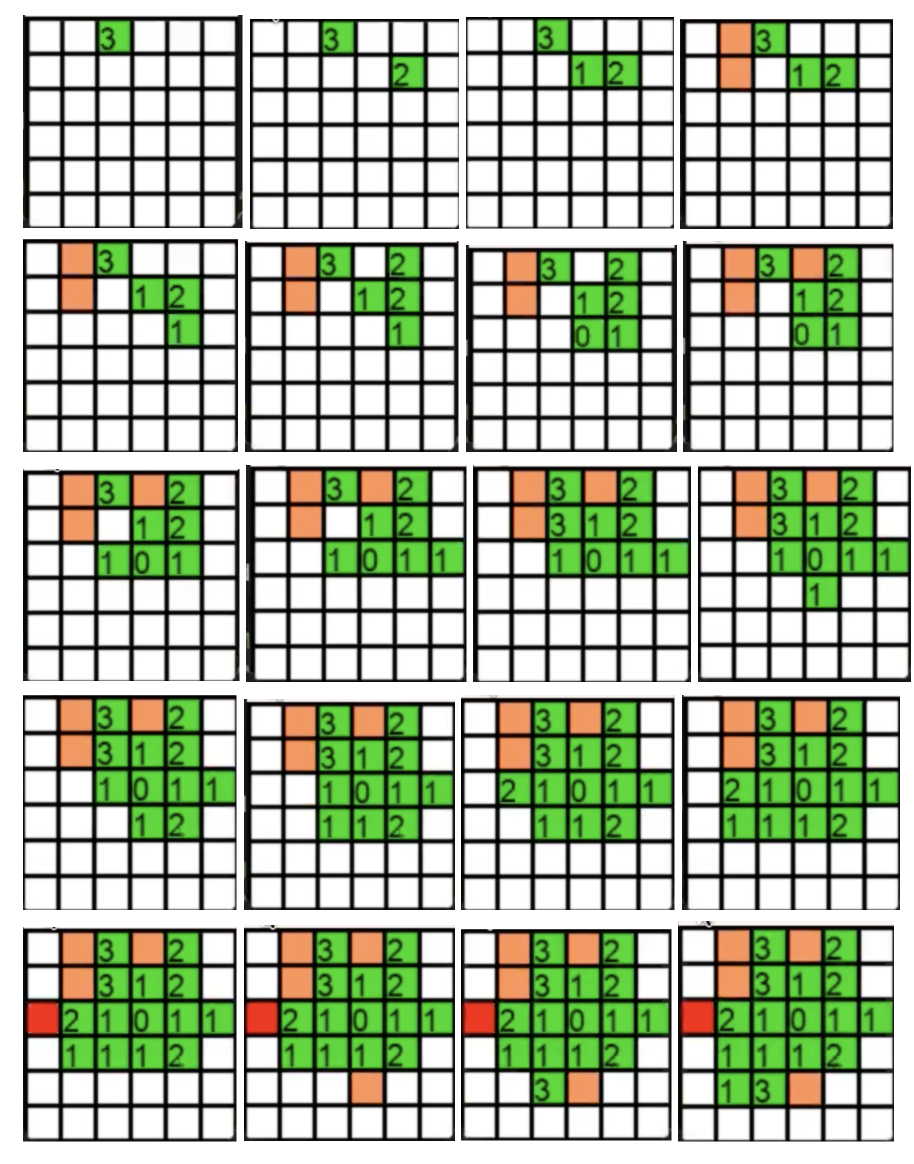
\includegraphics[width=0.6\textwidth]{images/perf_1.png}}{No Figure Yet}
    \IfFileExists{images/perf_2.png}{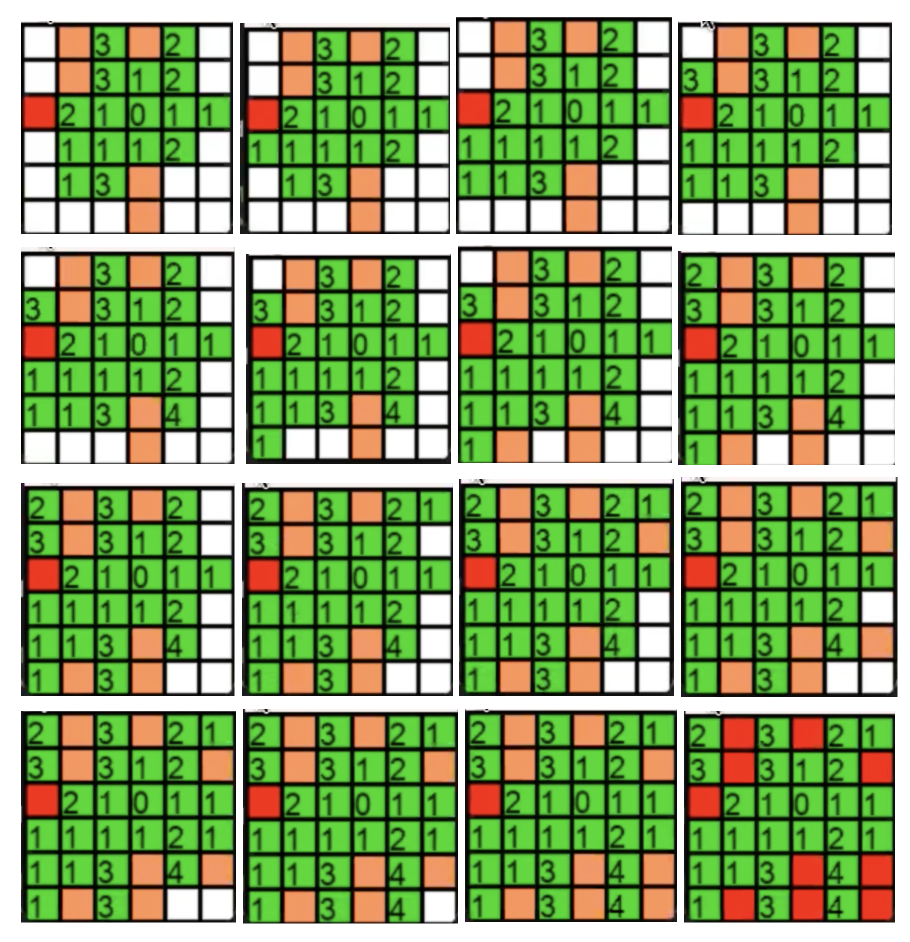
\includegraphics[width=0.6\textwidth]{images/perf_2.png}}{No Figure Yet}
	\end{figure}

	This is a play-by-play progression of the advanced agent from start to completion (left to right) of a 6x6 minesweeper board with 10 mines. The white cells indicate cells that have not been uncovered, the green cells are safe cells that have been uncovered with their clue displayed, the Orange cells are the cells that are inferred to be mines, and the red cells are mines that were incorrectly uncovered by the agent. The first 3 actions of the advanced agent are similar to basic because it picks randomly from the board however it becomes interesting at the 4th move. The agent inferred that 2 cells are mines, indicated as orange. This is different than the basic agent because the simple inference rules that the basic agent uses would not be able to infer these cells as mines. As you can see the agent continues to make advance inferences such as this. It uses the combination of multiple equations in the knowledge base to make these advance inferences. 
    There is one point where the algorithm queries a mine. It does this because it is forced to query a random cell because it cannot make anymore advanced inferences. If I were playing the game instead of choosing randomly I would choose a cell that are surrounded by smaller numbers such as 1’s so that it has a low probability of being a mine. Other than that there are not other decisions that surprised be or that I didn't’t agree with.

\end{solution}
\smallskip

\textbf{Performance: }
For a fixed, reasonable size of board, plot as a function of mine density the average final score (safely identified mines / total mines) for the simple baseline algorithm and your algorithm for comparison. This will require solving multiple random boards at a given density of mines to get good average score results.
Does the graph make sense / agree with your intuition? When does minesweeper become ‘hard’?
When does your algorithm beat the simple algorithm, and when is the simple algorithm better? Why?
How frequently is your algorithm able to work out things that the basic agent cannot?
\begin{solution} \hfill

    \begin{figure}[H]
	\centering
	\IfFileExists{images/performance_plot.png}{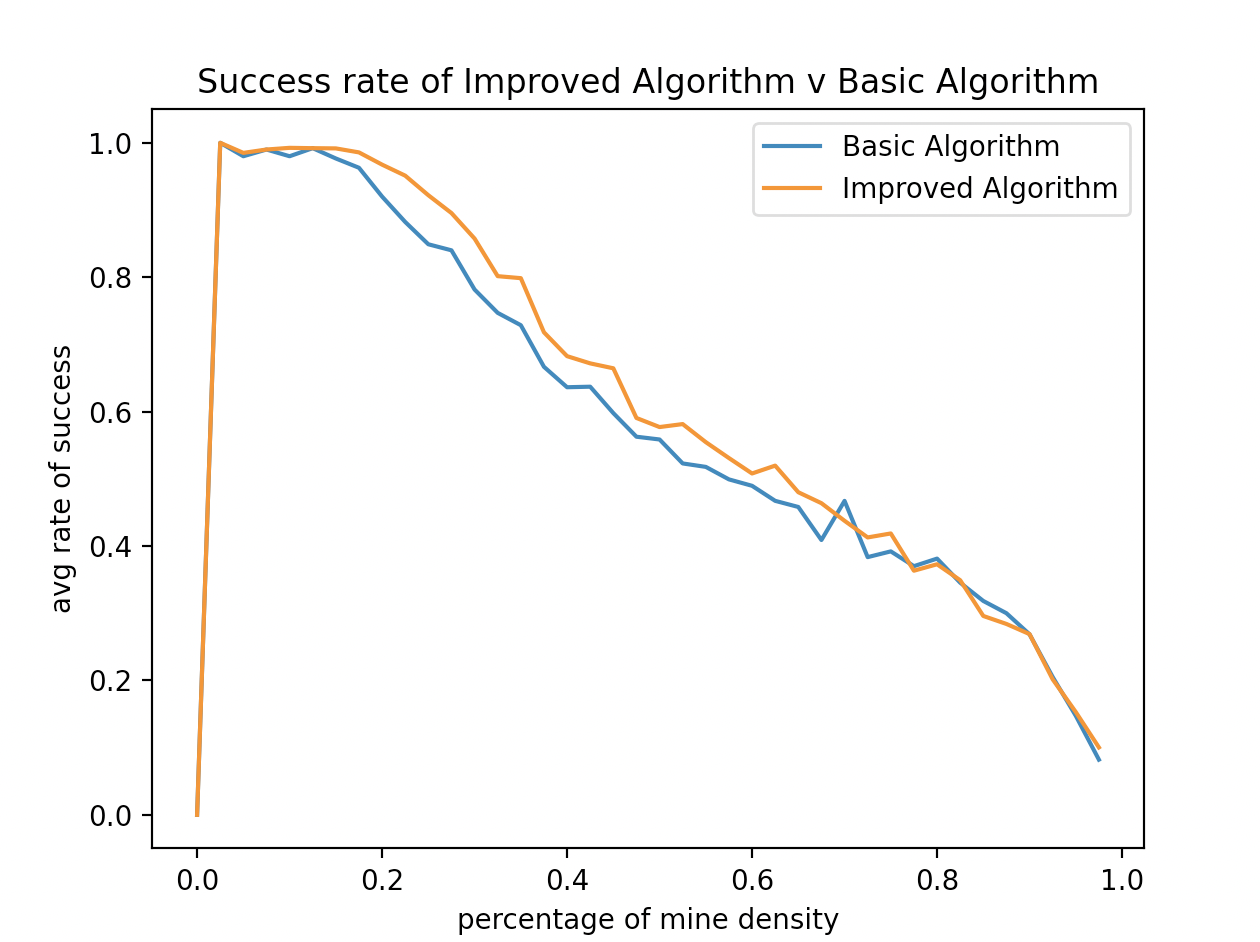
\includegraphics[width=0.7\textwidth]{images/performance_plot.png}}{No Figure Yet}
% 	\includegraphics[width=12cm]{dim100,50avg,step01}
	\caption{Plot of a function of mine density and the average final score for the baseline algorithm and our improved algorithm using a dimension of 20 and average of 10 random boards per given mine density}
	\end{figure}
	
    Minesweeper becomes 'hard' at greater mine densities, because that is the point when the algorithm will be less certain about the status of its surrounding cells and will have to pick randomly. Since the density of mines is greater, this increases the chances of randomly picking a mine. 
    \\\\
    The graph overall makes sense and is in accordance with our ideas regarding the improved algorithm being more accurate in identifying/ avoiding mines. 
    \\\\
    There are certain data points when the mine density increases where the basic algorithm performs slightly better. This could be attributed to being an anomaly because we are using an average of 10 grids at each mine density and this may not display the full breadth of our algorithm given one bad score has a very high impact on the overall average. \\
    This could also be attributed to the greater mine density. Since the improved algorithm gets inferences in a while loop where it gets every possible safe cell at any given moment, it leaves a greater density of mines in the uncovered cells it has to choose from when choosing randomly. This increases the chances of picking a mine since the density of mines in the remaining cells is greater. 
    \\\\
    The basic algorithm however does not reevaluate cells based on the current inferences until the next iteration so when it picks randomly it has a lower chance of picking a cell that is a mine.
    \\\\
    Overall, our improved algorithm performs better. Our algorithm is frequently able to work things out the basic algorithm cannot because our improved algorithm considers all the cells and their neighbors in relation to each other and not as individual entities. It combines the information from every uncovered cell to then make inferences about which cells are safe. 
	
\end{solution}
\smallskip

\textbf{Efficiency: }
What are some of the space or time constraints you run into in implementing this program? 
Are these problem specific constraints, or implementation specific constraints? 
In the case of implementation constraints, what could you improve on?
\begin{solution} \hfill \\
    Our improved agent works well with a board size of 20x20 and mine density of 30\% however when we increase that to 30x30 it is significantly slower.
    This problem is implementation specific and we could improve upon this by removing the various many deep copies we are performing. We perform a deep copy every time we update the knowledge base with the new inferences. This significantly increases the runtime and space so by removing it, we could improve the efficiency of our advanced agent.
\end{solution}

\smallskip

\textbf{Global Information: }
	Suppose you were told in advance how many mines are on the board. Include this in your knowledge base. How did you model this? Regenerate the plot of mine density vs average final score with this extra information, and analyze the results.
\begin{solution} \hfill \\
	\begin{figure}[H]
	\centering
	\IfFileExists{images/global_plot.png}{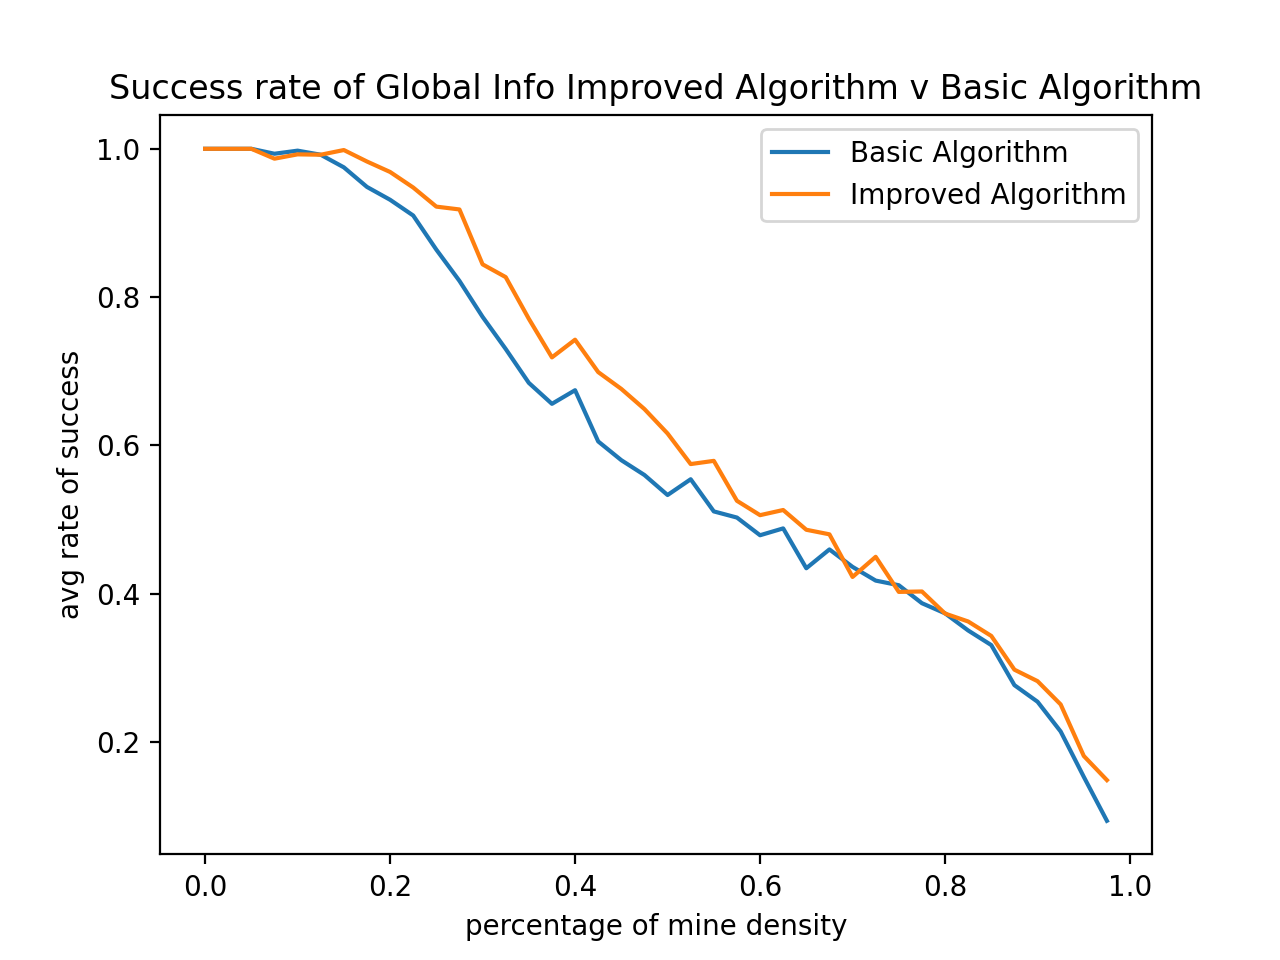
\includegraphics[width=0.7\textwidth]{images/global_plot.png}}{No Figure Yet}
	\caption{Plot of a function of mine density and the average final score for the baseline algorithm and our global information improved algorithm using a dimension of 20 and average of 10 random boards per given mine density}
	\end{figure}
	We modeled the idea of there being a known number of mines by adding it as an equation in our knowledge base. To do this, we added every cell on the board as part of the left-hand side of the equation and the number of mines on the right hand side. Since our knowledge base would be updated based on the cells uncovered, this equation added an additional data point that made our algorithm more precise. 
	\\\\
	Since the implementation of this idea was consistent with our algorithm it only made it quicker and more accurate in identifying mines. 
\end{solution}
\smallskip

\textbf{Better Decisions: }
	In both the basic and improved agent, when nothing more could be inferred, the agent selects a covered cell at random. Build a better selection mechanism. How can you justify it? Regenerate the plot of mine density vs average final score with improved cell selection, and analyze the results.
\begin{solution} \hfill \\
    To build a better selection mechanism we used our knowledge base to map out every possibility of a cell being a mine or a clue and used every single possibility to generate the probability of every uncovered cell being a mine. \\If a cell was a mine in every possibility, or was a clue in every possibility then we would add that to our list of identified cells. If we still do not have an assurance of a safe cell we go to the cell with the least probability of being a mine as long as it's probability is less than 0.3. If the least probability is greater than 0.3 then we choose a random cell from the cells not in knowledge (i.e. the cells we do not have a probability of). 
    
    $On$ $a$ $micro$ $scale,$ $it$ $may$ $look$ $like$ $this$: 
    \begin{tabbing}
    For the \=following board:\\
    \>[1] \=[A] \=[2] \\ 
    \>[B] \>[C] \>[D] \\
    \>[E] \>[3] \>[F] \\\\ 
    
    For which we have the following system of equations: \\
	\>A+B+C = 1 \\
	\>A+C+D = 2 \\
	\>E+B+C+D+F = 3\=\\
     \\\\
	
    We would assume A=0, based on this assumption we now have the following system:\\
    \>B+C = 1 \\
	\>C+D = 2 \\
	\>E+B+C+D+F = 3\=\\
    \\\\
    And through basic inference we have the following values: \\
    {A = 0, B = 0, C = 1, D = 1, E = ?, F = ?}
    \\\\
    So we as\=sume the next unknown value, to be 0. So based on the assumption that E=0, we have the following system: \\
    
	\>E+F = 1\=\\
    \\\\
    And through basic inference we have the following values: \\
    {A = 0, B = 0, C = 1, D = 1, E = 0, F = 1}\\
    This is now $one$ possibility of values. 
    \\\\
    We would go back to the last assumption and substitute that value with 1. Based on the assumption that E=1,\\ we have t\=he following system: \\
    \>E+F = 1\=\\
    \\\\
    And through basic inference we have the following values: \\
    {A = 0, B = 0, C = 1, D = 1, E = 1, F = 0}\\
    This is now a $second$ possibility of values. 
    \\\\
    We will once again go to the last assumption and substitute that value with 1. Based on the assumption that A=1,\\ we have \=the following system:\\
    
    \>B+C = 0 \\
	\>C+D = 1\\
	\>E+B+C+D+F = 3\=\\
     \\\\
    And through basic inference we have the following values: \\
    {A = 1, B = 0, C = 0, D = 1, E = 1, F = 1}\\
    This is now a $third$ possibility of values. \\\\
     
    The three possibilities of values we have are: \\\\
    \>{A = 0, B = 0, C = 1, D = 1, E = 0, F = 1}\\
    \>{A = 0, B = 0, C = 1, D = 1, E = 1, F = 0}\\
    \>{A = 1, B = 0, C = 0, D = 1, E = 1, F = 1}\\
    
    \\And we are able to compute the probability for each value being a mine as: \\
    {A = 1/3, B = 0, C = 2/3, D = 1, E = 2/3, F = 2/3}\\\\
    
    For which we will be able to identify B and D safely. If we had no values that were 0 or 1 we would explore the least \\probability if it were under 0.3.
     
    
    \end{tabbing}
\end{solution}

\textbf{Work Distribution}
\\
The work is our own and not copied or taken from any other students. 
\\\\
To work on this project we would meet up over video calls daily and discuss problems and our solutions. One person would then screen share and code while the others would contribute and also assist in coding using the request remote control feature in zoom. We would alternate in screen sharing and upload to git for version control. 
\\\\
The report was done similarly. We each took on a plot and a question to complete on our own. We then met to complete the rest as a group over video call. 
\\
$Asma$ $Makhdoom:$ Problem 2
\\
$Aamna$ $Farooq:$ Problem 3
\\
$Nada$ $Elshamaa:$ Problem 4 and Problem 6
\\
\smallskip

\end{document}